%%%%%%%%%%%%%%%%%%%%%%%%%%%%%%%%%%%%%%%%%
% Beamer Presentation
% LaTeX Template
% Version 1.0 (10/11/12) 
%
% This template has been downloaded from:
% http://www.LaTeXTemplates.com
%
% License:
% CC BY-NC-SA 3.0 (http://creativecommons.org/licenses/by-nc-sa/3.0/)
%
%%%%%%%%%%%%%%%%%%%%%%%%%%%%%%%%%%%%%%%%%

%----------------------------------------------------------------------------------------
%	PACKAGES AND THEMES
%----------------------------------------------------------------------------------------

\documentclass{beamer}

\mode<presentation> {
%\mode<handouts> {
%\mode<article> {


% The Beamer class comes with a number of default slide themes
% which change the colors and layouts of slides. Below this is a list
% of all the themes, uncomment each in turn to see what they look like.


%\usetheme{default}
%\usetheme{AnnArbor}
%\usetheme{Antibes}
%\usetheme{Bergen}
%\usetheme{Berkeley}
%\usetheme{Berlin}
%\usetheme{Boadilla}
\usetheme{CambridgeUS}
%\usetheme{Copenhagen}
%\usetheme{Darmstadt}
%\usetheme{Dresden}
%\usetheme{Frankfurt}
%\usetheme{Goettingen}
%\usetheme{Hannover}
%\usetheme{Ilmenau}
%\usetheme{JuanLesPins}
%\usetheme{Luebeck}
%\usetheme{Madrid}
%\usetheme{Malmoe}
%\usetheme{Marburg}
%\usetheme{Montpellier}
%\usetheme{PaloAlto}
%\usetheme{Pittsburgh}
%\usetheme{Rochester}
%\usetheme{Singapore}
%\usetheme{Szeged}
%\usetheme{Warsaw}

% As well as themes, the Beamer class has a number of color themes
% for any slide theme. Uncomment each of these in turn to see how it
% changes the colors of your current slide theme.

%\usecolortheme{albatross}
\usecolortheme{beaver}
%\usecolortheme{beetle}
%\usecolortheme{crane}
%\usecolortheme{dolphin}
%\usecolortheme{dove}
%\usecolortheme{fly}
%\usecolortheme{lily}
%\usecolortheme{orchid}
%\usecolortheme{rose}
%\usecolortheme{seagull}
%\usecolortheme{seahorse}
%\usecolortheme{whale}
%\usecolortheme{wolverine}

%\setbeamertemplate{footline} % To remove the footer line in all slides uncomment this line
%\setbeamertemplate{footline}[page number] % To replace the footer line in all slides with a simple slide count uncomment this line

%\setbeamertemplate{navigation symbols}{} % To remove the navigation symbols from the bottom of all slides uncomment this line
}

\usepackage{graphicx} % Allows including images
\graphicspath{{../figures}}
\usepackage{booktabs} % Allows the use of \toprule, \midrule and \bottomrule in tables
\usepackage{amsmath, amssymb, amsthm, gensymb,mathrsfs}%,eufrak}
\usepackage{hyperref}
\usepackage{tabularx}
\usepackage{longtable}
\usepackage{makecell}
\usepackage{multicol}
\usepackage{physics}

\newcommand{\uvec}[1]{\textbf{#1}}

\newcounter{excounter}
%\renewcommand{\thefpcounter}{\thechapter.\arabic{fpcounter}}
%\renewcommand{\thefpcounter}{\thesection.\arabic{fpcounter}}
\renewcommand{\theexcounter}{\arabic{excounter}}

\newtheorem{teorema}{Teorema}[section]
\newtheorem{definicio}{Definició}[section]

\usepackage[lastexercise]{exercise}

\graphicspath{{../figures}}

%----------------------------------------------------------------------------------------
%	 TITLE PAGE
%----------------------------------------------------------------------------------------

\title[Introduction]{Importing, summarizing and visualizing data} % The short title appears at the bottom of every slide, the full title is only on the title page

\author{Jordi Villà i Freixa} % Your name
\institute[FCTE] % Your institution as it will appear on the bottom of every slide, may be shorthand to save space
{
Universitat de Vic - Universitat Central de Catalunya \\
Study Abroad\\ % Your institution for the title page
\medskip
\textit{jordi.villa@uvic.cat} % Your email address
}
%\date{\today} % Date, can be changed to a custom date
\date{course 2023-2024}
\logo{
\includegraphics[width=.1\textwidth]{FCTE}}
\begin{document}

\begin{frame}
\titlepage % Print the title page as the first slide
\end{frame}

\begin{frame}
\frametitle{Índex} % Table of contents slide, comment this block out to remove it
\tableofcontents % Throughout your presentation, if you choose to use \section{} and \subsection{} commands, these will automatically be printed on this slide as an overview of your presentation
\end{frame}

%----------------------------------------------------------------------------------------
%	PRESENTATION SLIDES
%----------------------------------------------------------------------------------------

\begin{frame}
  \frametitle{Introduction to the course}
  The material in these slides is strongly based on \cite{kroese2020}. When other materials are going to be used, they will be cited accordingly.
  \end{frame}


%------------------------------------------------
\section{Python} % Sections can be created in order to organize your presentation into discrete blocks, all sections and subsections are automatically printed in the table of contents as an overview of the talk
%------------------------------------------------

\begin{frame}
  \frametitle{Python as the programming languange to learn}
  \begin{itemize}
    \item Easy to learn and powerful
    \item High-level efficient data structures
    \item Effective approach to object-orineted programming
    \item Interpreted
    \item Elegant syntax and \href{https://www.educative.io/answers/what-is-dynamic-typing}{dynamic typing}
  \end{itemize}
  The choice for rapid application development in many areas on most platforms:
  \begin{itemize}
    \item \href{https://docs.python.org/3/tutorial/index.html}{Official Python tutorial}
    \item \href{https://www.learnpython.org}{Interactive Python tutorial at LearnPython.org}
  \end{itemize}
\end{frame}

\begin{frame}
  \frametitle{Learning Python through Jupyter notebook and JupyterLab}
  \url{https://jupyter.org}
  \begin{itemize}
      \item Jupyter Notebook:
      \begin{itemize}
        \item web application
        \item creating and sharing computational documents
        \item several programming languages, including Python
        \item interactive output 
      \end{itemize}
      \item JupyterLab
      \begin{itemize}
        \item interactive development environment (IDE) for notebooks, code and data
        \item flexible interface
        \item modularity
      \end{itemize}
  \end{itemize}
\end{frame}

\begin{frame}[fragile]{Installing Jupyter}

  % We are going to rely on \href{https://docs.anaconda.com}{anaconda} or \href{https://conda.io/miniconda}{miniconda} to install software in our computer.

  % \begin{lstlisting}
  %   and       del     from    not    while 
  %   as        elif    global  or     with 
  %   assert    else    if      pass   yield 
  %   break     except  import  print 
  %   class     exec    in      raise 
  %   continue  finally is      return 
  %   def       for     lambda  try 
  %   \end{lstlisting}

  \begin{lstlisting}[language=bash,caption={installing and executing Jupyter notebook},frame=single]
  conda install jupyter
  jupyter notebook
\end{lstlisting}

\end{frame}
%------------------------------------------------
\section{Dealing with data} % Sections can be created in order to organize your presentation into discrete blocks, all sections and subsections are automatically printed in the table of contents as an overview of the talk
%------------------------------------------------

%\subsection{Subsection Example} % A subsection can be created just before a set of slides with a common theme to further break down your presentation into chunks


\begin{frame}
\frametitle{How is data stored?}
\begin{itemize}
  \item Data can be thought of as being the result of some random experiment.
  \item We are interested in analysing such data.
  \item The format is typically a set of variables or {\em features} as {\bf columns} while the different items are given as {\bf rows}.
  \item Typically the first columns represents a unique identifier or index.
  \item Some columns refer to the experimental settings and others are real variables.
  \item Many times variables and experimental designs are stored in two different files. The we call the experimental desgins file as the {\bf metadata} file, describing the details of the different experiments (or columns).  
\end{itemize}
\end{frame}

\begin{frame}{Data vs Metadata}
  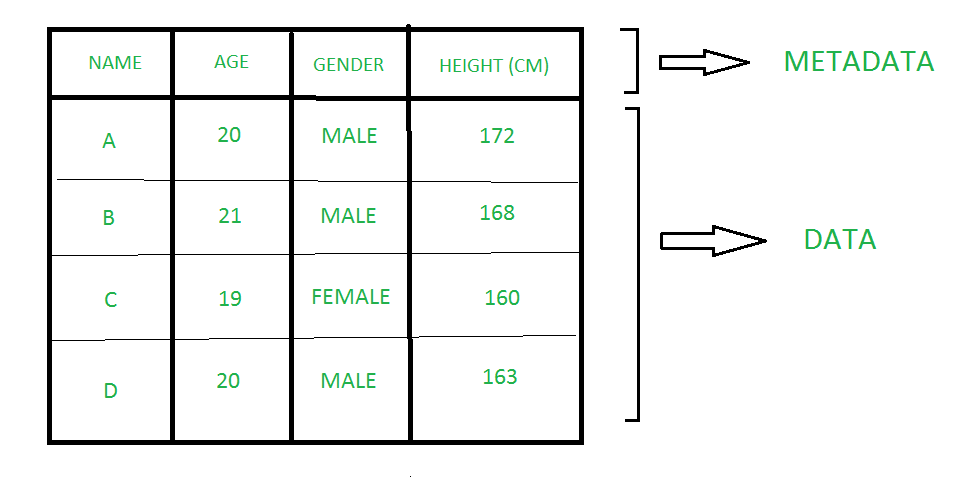
\includegraphics[width=\linewidth]{data_metadata}
\end{frame}
%------------------------------------------------

\begin{frame}
\frametitle{Training datasets}
There exist several datasets repositories that one can use to test the methods that are being developed. Some of them are going to be used in this course:
\begin{itemize}
\item Machine Learning Repository at University of California (\url{https://archive.ics.uci.edu})
\item Vincent Arel-Bundock repository (\url{https://vincentarelbundock.github.io/Rdatasets/})
\item Data from Pierre Lafaye de Micheaux and collaborators in their book  "The R Software. Fundamentals of Programming and Statistical Analysis" \cite{lafaye_de_micheaux_r_2013}
\end{itemize}
\end{frame}


\begin{frame}[allowframebreaks]
  \frametitle{EX 1}
  \begin{Exercise}[title={Data visualization}]
    Import the {\em EuStockMarkets} dataset from the Vincent Arel-Bundock repository. The data set contains the daily closing prices of four European stock indices during the
    1990s, for 260 working days per year.
    \begin{enumerate}
      \item Create a vector of times (working days) for the stock prices, between 1991.496 and 1998.646 with increments of 1/260.
      \item Reproduce Figure 1.10. [Hint: Use a dictionary to map column names (stock indices) to colors.]
     \end{enumerate}
     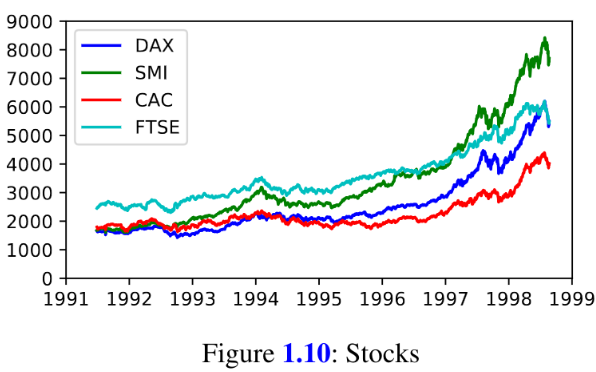
\includegraphics[width=0.9\linewidth]{stocks}
  \end{Exercise}
\end{frame}


%----------------------------------------------------------------------------------------
\section{Bibliography}
\bibliographystyle{plain}
\bibliography{DataSciencewithPython}

\end{document}
